\documentclass[11pt,a4paper]{article}
\usepackage{amsmath}
\usepackage{amsfonts}
\usepackage{amssymb}
\usepackage{fancyhdr}
\usepackage{lastpage}
\usepackage{graphicx}
\usepackage{ucs}
\usepackage[utf8x]{inputenc}
\usepackage[italian]{babel}
\usepackage[colorlinks=true,linkcolor=black]{hyperref}

\renewcommand{\headrulewidth}{0.6pt}
\renewcommand{\footrulewidth}{0.6pt}
% impostazione dello stile per le pagine interne del documento
\lhead{\leftmark}
\chead{}
\rhead{
\includegraphics[scale=0.15]{logo.png} }
\lfoot{Definizione di prodotto v0.1.0}
\cfoot{}
\rfoot{\thepage \ di \pageref{LastPage}}
% ridefinizione dello stile plain per il frontespizio
\fancypagestyle{plain}{
\fancyhf
}
% impostazione dello stile per l'indice
\fancypagestyle{indice}{
\lhead{\leftmark}
\chead{}
\rhead{
\includegraphics[scale=0.15]{logo.png}}
\lfoot{Definizione di prodotto v0.1.0}
\cfoot{}
\rfoot{}
}
\headheight = 46pt
%definizione del comando "\modfiche" per la creazione del diario delle modifiche
\newcommand{\modifiche} 
{
\newpage
\begin{center}
\textbf{Diario delle modifiche} \\
\bigskip
\begin{tabular}{|c|c|p{0.51\textwidth}|}
\hline
\textsc{Data} & \textsc{Versione} & \textsc{Modifica} \\
\hline
\hline
\textit{20 febbraio 2009} & 0.1.0 & Stesura dell'indice \\
\hline
\end{tabular}
\end{center}
}
%definizione del comando "\info" per la creazione delle informazioni del documento
\newcommand{\info} {
\bigskip
\begin{tabbing}
	\hspace*{0.3\textwidth} \= \hspace*{0.5\textwidth} \kill
	\parbox{0.3\textwidth}{\textbf{Verifica: }} \> \parbox{0.5\textwidth}{Verificatore} \\
	\parbox{0.3\textwidth}{\textbf{Approvazione: }} \> \parbox{0.5\textwidth}{Responsabile} \\
	\parbox{0.3\textwidth}{\textbf{Stato: }} \> \parbox{0.5\textwidth}{Preliminare | Formale} \\
	\parbox{0.3\textwidth}{\textbf{Uso: }} \> \parbox{0.5\textwidth}{Interno | Esterno} \\
	\parbox{0.3\textwidth}{\textbf{Distribuzione: }} \> \parbox{0.5\textwidth}{QuiXoft} \\
\end{tabbing}
}
%definizione del comando "\frontespizio" per la creazione del frontespizio
\newcommand{\frontespizio} {
\thispagestyle{plain}
\title{\begin{Huge}\textsc{Progetto SIGEOL}\end{Huge} \\ \textit{Definizione di prodotto \\ v0.1.0}}
\author{Redazione: }
\maketitle
\medskip
\begin{center}

\includegraphics[scale=0.5]{logo.png} \\
\textit{quixoft.sol@gmail.com}
\end{center}
\medskip
\info
\begin{center}
\textbf{Sommario} \\
Descrizione dettagliata delle caratteristiche tecniche ed architetturali del prodotto \textsc{Sigeol}
\end{center}
\newpage
}
%definizione del comando "\indice" per la creazione dell'indice
\newcommand{\indice} {
\thispagestyle{indice}
\tableofcontents
\newpage
}
\pagestyle{fancy}
\begin{document}
\frontespizio
\indice
\setcounter{page}{1}
\section{Introduzione}
\subsection{Scopo del documento}
Il presente documento denominato \textsc{Descrizione di prodotto} si prefigge di illustrare ed analizzare con maggior dettaglio i metodi ed i formalismi adottati nella definizione del prodotto \textsc{Sigeol}
\subsection{Scopo del prodotto}
Il progetto sotto analisi, denominato \textsc{Sigeol}, si prefigge di automatizzare la generazione, la gestione, l’ottimizzazione e la consultazione degli orari di lezione. Per maggiori dettagli consultare il documento denominato \textsc{Analisi dei Requisiti} alla sua ultima versione.
\subsection{Glossario}
Le definizioni dei termini specialistici usati nella stesura di questo e di tutti gli altri documenti possono essere trovate nel documento denominato \textsc{Glossario} al fine di eliminare ogni ambiguità e di facilitare la comprensione dei temi trattati. Ogni termine la cui definizione è disponibile all’interno del glossario verrà marcato con una sottolineatura.
\subsection{Riferimenti normativi}
Il documento denominato \textsc{Norme di Progetto} accompagna e complementa il presente ed ogni documento ufficiale.

\section{Standard di progetto}
\subsection{Standard di progettazione architetturale}
La definizione dell'intero sistema oggetto di studio è stata effetuata attraverso l'uso di diagrammi UML e l'applicazione di pattern consolidati ed in uso in molti prodotti software.
\subsubsection{UML}
Il linguaggio UML è utilizzato per la modellazione architetturale di un sistema in quanto grazie alla sua capacità e chiarezza espressiva risulta di facile comprensione anche a persone esterne al progetto stesso. Il team QuiXoft ha utilizzato UML 2.0 per:
\begin{itemize}
 \item Diagrammi use-case nel documento \textsc{Analisi dei Requisiti}
 \item Diagrammi delle classi, delle componenti, di attività e delle sequenze nei documenti \textsc{Specifica tecnica} e \textsc{Definizione di prodotto}
\end{itemize}
\subsection{Pattern}
All'interno dell'architettura del sistema sono stati utilizzati i seguenti pattern, presenti nel \underline{framework} Ruby on Rails il quale è alla base di tutto il prodotto:
\begin{description}
 \item[\textbf{MVC}] 
Il \underline{pattern} MVC (Model View Controller) si basa sulla separazione tra i componenti software del sistema, che gestiscono il modo in cui presentare i dati, e i componenti che gestiscono i dati stessi. 
 \item[\textbf{Façade}]
Permette, attraverso un'interfaccia più semplice, l'accesso a sottosistemi aventi interfacce complesse e molto diverse tra loro, nonché a blocchi di codice complessi.
\item[\textbf{REST}]
Representational state transfer (REST) è un tipo di architettura software per i sistemi di ipertesto distribuiti come il World Wide Web. 
REST si riferisce ad un insieme di principi di architetture di rete, i quali delineano come le risorse sono definite e indirizzate.

\item[\textbf{Convention Over Configuration}]
Convention Over Configuration è un paradigma di programmazione che prevede configurazione minima (o addirittura assente) per il programmatore che utilizza un \underline{framework} che lo rispetti, obbligandolo a configurare solo gli aspetti che si differenziano dalle implementazioni standard o che non rispettano particolari convenzioni di denominazione o simili.
Significa che Rails prevede delle impostazioni di default per qualsiasi aspetto dell’applicazione. Utilizzando queste convenzioni sarà possibile velocizzare i tempi di sviluppo evitando di realizzare scomodi file di configurazione. L’esempio più chiaro del COC si può notare a livello di modelli: rispettando le convenzioni previste dal \underline{framework} è possibile realizzare strutture di dati complesse con molte relazioni tra oggetti in pochissimo tempo, in maniera quasi meccanica e soprattutto senza definire nessuna configurazione. Questo concetto differenzia Rails dai \underline{framework} che prevedono molte righe di configurazione per ogni aspetto dell’applicazione. Con il COC tutto diventa più snello e più dinamico. Ovviamente per situazioni in cui le convenzioni non possano essere rispettate, Rails permette di utilizzare schemi funzionali diversi da quelli previsti.
\item[\textbf{DRY}]
Questo concetto, fortemente filosofico, prevede che ciascun elemento di un’applicazione debba essere implementato solamente una volta e niente debba essere ripetuto. Questo significa che, mediante Rails, è possibile gestire funzionalità ripetitive con una estrema fattorizzazione del codice (''scrivo una volta e uso più volte'') che facilita sia lo sviluppo iniziale che eventuali modifiche successive del prodotto.
\item[\textbf{View Helper}]
Questo \underline{pattern} disaccoppia il Business Logic dallo strato View, il che facilita
la manutenibilità. Aiuta a separare, in fase di sviluppo, la responsabilità
del web designer e dello sviluppatore.
\item[\textbf{Active Record}]
Secondo il \underline{pattern} Active Record esiste una relazione molto stretta fra tabella e classe, colonne e attributi della classe. 
\begin{itemize}
 \item una tabella di un \underline{database} relazionale è gestita attraverso una classe
\item una singola istanza della classe corrisponde ad una riga della tabella
\item alla creazione di una nuova istanza viene creata una nuova riga all'interno della tabella, e modificando l'istanza la riga viene aggiornata
\end{itemize}
\end{description}

\subsection{Standard di documentazione del codice}
Il team QuiXoft si avvalerà dello strumento \underline{RDoc}, specifico per il linguaggio Ruby. Questo strumento estrapola dal codice sorgente i commenti al codice stesso, organizzandoli e rendendoli disponibili alla consultazione tramite pagine HTML. Per questo motivo ogni membro del team alla stesura di qualsiasi classe o metodo dovrà documentarlo tramite la sintassi specifica di RDoc.

\subsection{Standard di denominazione di entità e relazioni}
Lo schema di denominazione deve essere determinante per la comprensione del flusso logico dell'applicazione. Verrano quindi utilizzati nomi significativi che identifichino la funzione e lo scopo dell'elemento. Inoltre saranno seguite le convenzioni generali dello specifico linguaggio di programmazione utilizzato per realizzare l'elemento, nonchè ulteriori convenzioni dettate dal framework utilizzato. Per maggiori informazioni consultare la sezione \ref{programmazione}

\subsection{Standard di programmazione}\label{programmazione}
Ogni file deve contenere esattamente una classe od un modulo, eccezion fatta per i \underline{template} di file HTML e JavaScript. Inoltre è necessaria ai fini di una migliore leggibilità, l'uso di una corretta indentazione, fornita dall'ambiente di sviluppo. 
\subsubsection{Ruby e framework Rails}
Di seguito sono elencate le convenzioni utilizzate negli elementi sviluppati con il linguaggio Ruby.
\subsubsection*{Variabili locali}
Prima lettera minuscola, seguita da altri caratteri minuscoli. Se la variabile comprende più parole, queste andranno separate con un \_ (underscore). Esempio: \verb|variabile_locale|
\subsubsection*{Variabili d'instanza}
Si utilizza la stessa convenzione adottata nelle variabili locali, con l'aggiunta di un @ (at) prima del nome. Esempio: \verb|@variabile_istanza|
\subsubsection*{Variabili di classe}
Si utilizza la stessa convenzione adottata nelle variabili locali, con l'aggiunta di una doppia @ (at) prima del nome. Esempio: \verb|@@variabile_classe|
\subsubsection*{Variabili globali}
Si utilizza la stessa convenzione adottata nella variabili locali, con l'aggiunta di un \verb|$| (dollar) prima del nome. Esempio: \verb|$variabile_globale|
\subsubsection*{Costanti}
Prima lettera maiuscola, seguita da altri caratteri maiuscoli. Se la variabile comprende più parole, queste andranno separate con un \_ (underscore). Esempio: \verb|UNA_COSTANTE|
\subsubsection*{Metodi d'istanza}
Prima lettera minuscola, seguita da altri caratteri minuscoli. Se il nome comprende più parole, queste andranno separate con un \_ (underscore). Esempio: \verb|metodo_istanza|
\subsubsection*{Classi e moduli}
Prima lettera maiuscola, seguita da altri caratteri minuscoli. Se il nome comprende più parole, la prima lettera di ogni parola deve essere maiuscola. Esempio: \verb|UnaClasse|
\subsubsection*{Model}
Si utilizza la stessa convenzione per le classi ed inoltre il nome dovrà essere il singolare (in lingua inglese) del nome della tabella del database a cui si riferisce. Esempio: \verb|Order|
\subsubsection*{Controller}
Si utilizza la stessa convenzione per le classi ed inoltre il nome dovrà essere il plurale (in lingua inglese) del nome del Model a cui si riferisce, seguito dalla parola \textit{Controller}. Esempio: \verb|OrdersController|
\subsubsection*{Tabelle del database}
Prima lettera minuscola, seguita da altri caratteri minuscoli. Se il nome comprende più parola, queste andranno separate con un \_ (underscore). Inoltre il nome deve essere il plurale del model (in lingua inglese) a cui la tabella si riferisce. Esempio: \verb|orders|
\subsubsection*{Chiave primaria}
Il nome della chiave primaria dovrà essere \verb|id|
\subsubsection*{Chiavi esterne}
Il nome della chiave esterna dovrà essere il singolare (in lingua inglese) della tabella di riferimento, seguito da un \_ (underscore) e dalla parola \textit{id}, con ogni carattere minuscolo. Esempio: \verb|order_id|
\subsubsection*{Tabelle per le relazioni molti a molti}
Concatenazione tramite \_ (underscore) dei nomi al plurale (in lingua inglese) dei model coinvolti in ordine alfabetico, con ogni carattere minuscolo. Esempio \verb|items_orders|
\subsubsection*{File}
Ogni nome di file è caratterizzato dalla presenza di soli caratteri minuscoli e la concatenazione di più parole è effettuata tramite \_ (underscore).
\subsubsection{Java}
Per quanto riguarda i file sorgenti scritti utilizzando il linguaggio Java fanno fede le norme e convenzioni acquisite da ogni membro del team durante il corso di Programmazione 3 o Programmazione concorrente e distribuita, a seconda dell'ordinamento a cui il componente appartiene.

\subsection{Strumenti di lavoro}
Durante tutto lo svolgimento del progetto, il team QuiXoft utilizzarà i seguenti strumenti:
\begin{itemize}
 \item IDE NetBeans 6.5 \\ \textit{http://www.netbeans.org/}
 \item JDK 6 Update 12 \\ \textit{http://java.sun.com/}
 \item JRuby 1.1.5 \\ \textit{http://jruby.codehaus.org/}
 \item GlassFishV3 \\ \textit{https://glassfish.dev.java.net/}
 \item MySql 5.0 \\ \textit{http://www.mysql.com/}
 \item Rails framework \\ \textit{http://rubyonrails.org/}
 \item RDoc \\ \textit{http://rdoc.sourceforge.net/}
 \item rcov \\ \textit{http://rubyforge.org/projects/rcov/}
 \item W3C validator \\ \textit {http://validator.w3.org/}
 \item Prototype 1.6 \\ \textit {http://www.prototypejs.org/}
 \item \LaTeX \\ \textit {http://www.latex-project.org/}
\end{itemize}

\section{Specifica delle componenti}
Il sistema Sigeol è strutturato seguendo il paradigma MVC, con l'aggiunta di ulteriori: Helper, MiddleMan e Algorithm.
\subsection{Componente Model} \label{model}
\subsection{Componente Controller}
La componente Controller si occupa di gestire le azioni che l'utente effettua, solitamente attraverso una view. Ogni metodo pubblico rappresenta quindi una specifica azione, eccezion fatta per l'Application Controller.
Di seguito è riportato il diagramma delle classi che illustra questa componente. Sono stati omessi volutamente i tipi di ritorno per i metodi che implementano un'azione, in quanto queste operazioni non sono utilizzate per restituire un valore, bensì inizializzano alcune variabili d'istanza che saranno successivamente disponibili nella view specifica per quella azione. Inoltre per aumentare la leggibilità è stata omessa la derivazione della classe \verb|ApplicationController| da \verb|ActionController::Base|. \\
\bigskip \\
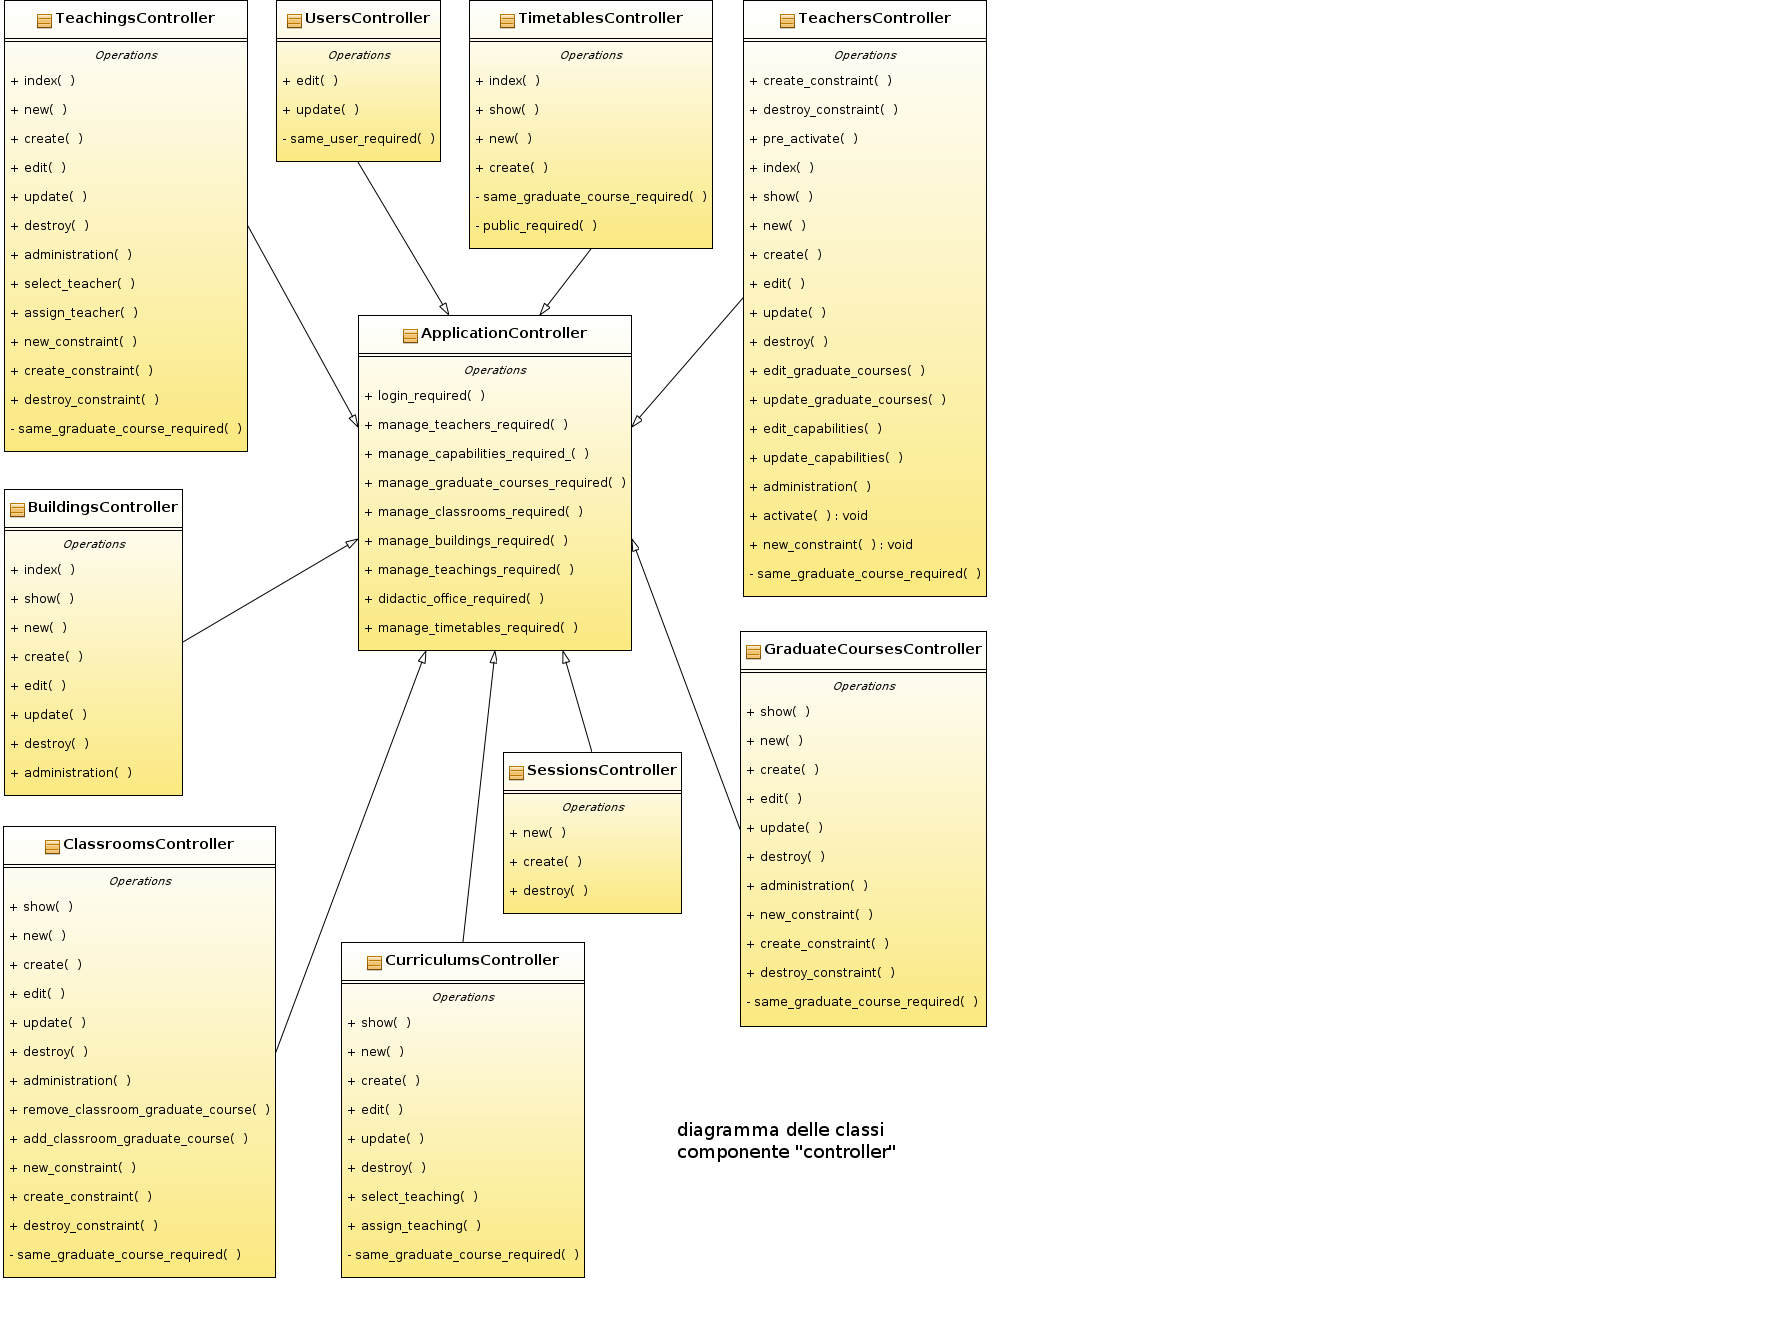
\includegraphics[scale=0.34]{images/Controller_ClassDiagram.png}
\subsubsection{Azioni comuni a più controller}
Per evitare fastidiose ripetizioni in questa sezione verranno descritti i metodi che figurano con lo stesso nome in diversi controller. La scelta dello stesso nome non è casuale, in quanto rispecchia la funzione dell'azione.
\begin{itemize}
 \item \verb|index|: rende disponibile alla view specifica un insieme d'istanze ed è raggiungibile eseguendo una richiesta GET all'indirizzo /nomecontroller. Ad esempio l'azione \verb|index| di \verb|GraduateCourseController| fornisce alla view un insieme di corsi di laurea ed è raggiungibile attraverso una richiesta GET all'indirizzo /graduate\_courses.
 \item \verb|show|: rende disponibile alla view specifica un'istanza ed è raggiungibile eseguendo una richiesta GET all'indirizzo /nomecontroller/id. Usando sempre l'esempio dei corsi di laurea, eseguendo una richiesta GET all'indirizzo /graduate\_courses/1 verranno visualizzate le informazioni relative al corso di laurea con id 1.
 \item \verb|new|: rende disponibile alla view specifica un'istanza vuota per permettere l'inserimento di un nuovo oggetto. E' raggiungibile eseguendo una richiesta GET /nomecontroller/new
 \item \verb|create|: acquisisce i dati da una richiesta POST per salvare l'oggetto nel database attraverso il model. Solitamente i dati provengono da una form con metodo POST presente nella view per l'azione \verb|new|. E' possibile comunque invocare questa azione mediante una richiesta POST all'indirizzo /nomecontroller
 \item \verb|edit|: rende disponibile alla view specifica un'istanza esistente per permetterne la modifica. e' raggiungibile attraverso una richiesta GET all'indirizzo /nomecontroller/id/edit
 \item \verb|update|: acquisisce i dati da una richiesta PUT per aggiornare lo stato dell'oggetto nel database attraverso il model. Solitamente i dati provengono da una form con metodo PUT presente nella view per l'azione \verb|edit|. E' possibile comunque invocare questa azione mediante una richiesta PUT all'indirizzo /nomecontroller/id
 \item \verb|destroy|: distrugge l'oggetto attraverso il model. Questa azione viene invocata tramite una richiesta DELETE all'indirizzo /nomecontroller/id
 \item \verb|administration|: rende disponibile alla view specifica un insieme d'istanze per effettuarne l'amministrazione. Questa azione è raggiungibile attraverso una richiesta GET all'indirizzo \\ /nomecontroller/administration.
 \item \verb|new_constraint|: rende disponibile alla view specifica un'istanza per un vincolo od una preferenza per permetterne l'inserimento. E' raggiungibile eseguendo una richiesta GET all'indirizzo \\ /nomecontroller/id/new\_constraint
 \item \verb|create_constraint|: acquisisce i dati da una richiesta POST per salvare il vincolo o la preferenza nel database attraverso il model. Solitamente i dati provengono da una form con metodo POST presente nella view per l'azione \verb|new_constraint|. E' possibile comunque invocare questa azione mediante una richiesta POST all'indirizzo /nomecontroller/id/create\_constraint
 \item \verb|destroy_constraint|: distrugge l'oggetto attraverso il model. Questa azione viene invocata tramite una richiesta DELETE all'indirizzo /nomecontroller/id/destroy\_contraint/id
\end{itemize}
Non è necessaria l'autenticazione o il possesso di alcuni privilegi per eseguire le azioni \verb|index| e \verb|show|. Per quanto riguarda gli altri metodi, invece, può ritenersi necessaria l'autenticazione od il possesso di alcuni privilegi. Per ogni controller sarà descritto questo aspetto.
Differente invece è il caso del metodo \verb|same_graduate_course_required|, dichiarato privato nei controllers che lo implementano. Questo metodo non rispecchia un'azione, ma è utilizzato come filtro, ovvero è chiamato prima o dopo una determinata azione, per impedire la modifica o la cancellazione di un oggetto appartenente ad un corso di laurea diverso da quello dell'utente autenticato.
\subsubsection{ApplicationController}
Questa classe deriva direttamente da \verb|ActionController::Base|, ed è estesa da ogni controller. Prevede metodi di pubblica utilità per gli altri controller, ma nessuna azione. L' \verb|ApplicationController| del sistema Sigeol prevede i seguenti metodi pubblici, utilizzati come filtri dagli altri controller.
\begin{itemize}
 \item \verb|login_required|: se l'utente non è autenticato questo metodo reindirizza alla pagina di login
 \item \verb|manage_teachers_required|: se l'utente non possiede i privilegi per gestire i docenti questo metodo reindirizza alla pagina principale mostrando un errore.
 \item \verb|manage_capabilities_required|: se l'utente non possiede i privilegi per gestire i privilegi questo metodo reindirizza alla pagina principale mostrando un errore.
 \item \verb|manage_graduate_courses_required|: se l'utente non possiede i privilegi per gestire i corsi di laurea questo metodo reindirizza alla pagina principale mostrando un errore.
 \item \verb|manage_classrooms_required|: se l'utente non possiede i privilegi per gestire le aule questo metodo reindirizza alla pagina principale mostrando un errore.
 \item \verb|manage_buildings_required|: se l'utente non possiede i privilegi per gestire gli edifici questo metodo reindirizza alla pagina principale mostrando un errore.
 \item \verb|manage_teachings_required|: se l'utente non possiede i privilegi per gestire gli insegnamenti questo metodo reindirizza alla pagina principale mostrando un errore.
 \item \verb|manage_timetables_required|: se l'utente non possiede i privilegi per gestire gli orari questo metodo reindirizza alla pagina principale mostrando un errore.
 \item \verb|didactic_office_required|: se l'utente non appartiene ad una segreteria didattica questo metodo reindirizza alla pagina principale mostrando un errore.
\end{itemize}
\subsubsection{GraduateCoursesController}
Il controller \verb|GraduateCourseController| permette alla segreteria didattica di creare e eliminare i corsi di laurea. Inoltre permette agli utenti con gli opportuni privilegi di aggiornare le informazioni relative ai propri corsi di laurea.
I filtri utilizzati in questo controller vengono tutti anteposti alle azioni e sono i seguenti:
\begin{itemize}
 \item \verb|login_required| non è utilizzato nelle azioni \verb|index| e \verb|show|
 \item \verb|manage_graduate_courses_required| è utilizzato nelle azioni \verb|edit|, \verb|update|, \verb|destroy|, \verb|administration|
 \item \verb|didactic_office_required| è utilizzato nelle azioni \verb|new|, \verb|create| e \verb|destroy|
 \item \verb|same_graduate_course_required| è utilizzato nelle azioni \verb|edit|,\\ \verb|update|, e \verb|destroy|.
\end{itemize}
\subsubsection{CurriculumsController}
Il controller \verb|CurriculumsController| permette all'utente con gli opportuni privilegi di creare, modificare ed eliminare le informazioni relative ai curricula dei propri corsi di laurea, nonchè di aggiungere o rimuove insegnamenti da quest'ultimi attreverso i metodi \verb|select_teaching|, raggiungibile medianta una richiesta GET all'indirizzo /curriculums/id/select\_teaching, e \verb|assign_teaching|, raggiungibile mediante una richiesta POST all'indirizzo /curriculums/id/assign\_teaching. Il primo fornisce alla view una lista degli insegnamenti presenti nel corso di laurea a cui il curriculum appartiene, mentre il secondo crea questa associazione tramite il model.
I filtri utilizzati in questo controller vengono tutti anteposti alle azioni e sono i seguenti:
\begin{itemize}
 \item \verb|login_required| non è utilizzato solamente nell'azione \verb|show|
 \item \verb|manage_graduate_courses_required| non è utilizzato solamente nell'azione \verb|show|
 \item \verb|same_graduate_course_required| è utilizzato nelle azioni \verb|edit|,\\ \verb|update|, \verb|select_teaching| e \verb|assign_teaching|.
\end{itemize}
\subsubsection{UsersController}
Il controller \verb|UsersController| dispone solamente delle azioni \verb|edit| e \verb|update| e del metodo privato \verb|same_user_required| (utilizzato come filtro anteposto alle due azioni assieme al filtro \verb|login_required|). Questa scelta progettuale deriva dalla relazione tra i model \verb|Teacher|, \verb|DidacticOffice| e \verb|User|. Confrontare la sezione \ref{model}.
Il metodo privato \verb|same_user_required| garantisce che non si stia cercando di modificare un utente diverso dal proprio.
\subsubsection{TeachersController}
Il controller \verb|TeachersController| permette all'utente con gli opportuni privilegi di creare, modificare ed eliminare i docenti dei propri corsi da laurea, nonchè di attribuire ad essi nuovi privilegi e corsi di laurea. Attraverso l'azione \verb|new| viene rischiesto un indirizzo e-mail di un docente e l'azione \verb|create| verificherà se questo è presente o meno nel database. Nel primo caso se il docente appartiene già a quel corso di laurea verrà segnalato un errore, altrimenti verrà aggiunto; nel secondo caso verrà inviata al nuovo docente una mail con le istruzioni per la registrazione al sistema. Il nuovo docente tramite l'azione \verb|pre_activate|, raggiungibile mediante una richista GET all'indirizzo /teachers/id/pre\_activate?digest=, potrà completare la creazione dello proprio user, e del relativo indirizzo, che sarà delegata all'azione \verb|activate|, raggiungibile mediante una richiesta POST all'indirizzo /teachers/id/activate?digest=. La certezza che solamente il docente invitato potrà creare il proprio account è resa possibile tramite il parametro \verb|digest| che solamente chi ha ha ricevuto la mail di invito può conoscere.

Infine attraverso le azioni \verb|edit_graduate_courses|, \verb|edit_capabilities|, \verb|update_graduate_courses| e \verb|update_capabilities|, raggiungibili rispettivamente mediante una richiesta GET all'indirizzo \\ /teachers/id/edit\_graduate\_courses o /teachers/id/edit\_capabilities e mediante una richiesta POST all'indirizzo /teachers/is/update\_graduate\_courses o /teachers/id/update\_capabilities, è possibilile modificare o rimuovere corsi di laurea e privilegi ai docenti da user che ne hanno la facoltà.
I filtri utilizzati in questo controller vengono tutti anteposti alle azioni e sono i seguenti:
\begin{itemize}
 \item \verb|login_required| non è utilizzato nelle azioni \verb|index|, \verb|show| ed \verb|activate|
 \item \verb|manage_teachers_required|  è utilizzato nelle azioni \verb|new|, \verb|create|,\\ \verb|administration|, \verb|edit_graduate_courses|, \verb|update_graduate_courses|
 \item \verb|manage_capabilities_required| è utilizzato nelle azioni \\ \verb|edit_capabilities| e \verb|update_capabilities|
 \item \verb|same_graduate_course_required| è utilizzato nelle azioni \\ \verb|edit_graduate_courses|, \verb|edit_capabilities|,\\ \verb|update_graduate_courses| e \verb|update_capabilities|.
\end{itemize}
\subsubsection{SessionsController}
Il controller \verb|SessionsController| permette la creazione di una sessione al momento dell'autenticazione dello user. Utilizza quindi le azioni \verb|new|, \verb|create| e \verb|destroy| senza alcun filtro, raggiungibili rispettivamente con una richiesta GET all'indirizzo /session/new, POST all'indirizzo /session e DELETE all'indirizzo /session/id.
\subsubsection{TeachingsController}
Il controller \verb|TeachingsController| permette all'utente con gli opportuni privilegi di creare, modificare ed eliminare le informazioni relative agli insegnamenti dei propri corsi di laurea, nonchè di aggiungere o rimuove il docente che tiene l'insegnamento in questione attraverso le azioni \verb|select_teacher|, raggiungibile medianta una richiesta GET all'indirizzo \\ /teachings/id/select\_teacher, e \verb|assign_teacher|, raggiungibile mediante una richiesta POST all'indirizzo /teachers/id/assign\_teacher. Il primo fornisce alla view una lista dei docenti presenti nel corso di laurea a cui il curriculum appartiene, mentre il secondo crea questa associazione tramite il model.
I filtri utilizzati in questo controller vengono tutti anteposti alle azioni e sono i seguenti:
\begin{itemize}
 \item \verb|login_required| non è utilizzato nelle azioni \verb|index| e \verb|show|
 \item \verb|manage_teachings_required| non è utilizzato nelle azioni \verb|index| e \verb|show|
 \item \verb|same_graduate_course_required| è utilizzato nelle azioni \verb|edit|,\\ \verb|update|, \verb|destroy|, \verb|select_teacher| e \verb|assign_teacher|.
\end{itemize}
\subsubsection{BuildingsController}
Il controller \verb|BuildingsController| permette all'utente con gli opportuni privilegi di creare, modificare ed eliminare le informazioni relative agli edifici ed ai relativi indirizzi.
I filtri utilizzati in questo controller vengono tutti anteposti alle azioni e sono i seguenti:
\begin{itemize}
 \item \verb|login_required| non è utilizzato nelle azioni \verb|index| e \verb|show|
 \item \verb|manage_buildings_required| non è utilizzato nelle azioni \verb|index| e \verb|show|
\end{itemize}
Non è presente il filtro \verb|same_graduate_course_required| in quanto un edificio non appartiene ad uno o più corsi di laurea, bensì all'intero sistema universitario.
\subsubsection{ClassroomsController}
Il controller \verb|ClassroomsController| permette all'utente con gli opportuni privilegi di creare, modificare ed eliminare le informazioni relative alle aule, nonchè di aggiungere o rimuovere le aule ai propri corsi di laurea attraverso le azione \verb|add_classroom_graduate_course| e \\ \verb|remove_classroom_graduate_course| raggiungibili attraverso una richiesta POST agli indirizzi, rispettivamente,\\ /classrooms/id/add\_classroom\_graduate\_course e \\ /classrooms/id/remove\_classroom\_graduate\_course
I filtri utilizzati in questo controller vengono tutti anteposti alle azioni e sono i seguenti:
\begin{itemize}
 \item \verb|login_required| non è utilizzato solamente nell'azione \verb|show|
 \item \verb|manage_classrooms_required| non è utilizzato solamente nell' azione \verb|show|
 \item \verb|same_graduate_course_required| non è utilizzato nelle azioni \verb|show|, \verb|new| e \verb|create|
\end{itemize}
\subsubsection{TimetablesController}
Il controller \verb|TimetablesController| permette all'utente con gli opportuni privilegi di creare ed eliminare gli orari.
I filtri utilizzati in questo controller vengono tutti anteposti alle azioni e sono i seguenti:
\begin{itemize}
 \item \verb|login_required| non è utilizzato nelle azioni \verb|index| e \verb|show|
 \item \verb|manage_timetables_required| non è utilizzato nelle azione \verb|index| e \verb|show|
 \item \verb|same_graduate_course_required| non è utilizzato nelle azioni \verb|index|, \verb|show|, \verb|new|, \verb|create|
 \item \verb|public_required| è utilizzato nell'azione \verb|show| ed assicura che l'orario che si intente visualizzare sia stato dichiarato pubblico da un utente con gli opportuni privilegi.
\end{itemize}
\subsection{Componente View}
Il componente View si occupa di presentare le informazioni presenti nel sistema a chiunque le richieda, sia esso un utente finale o un altro sistema software. Per far ciò sono presenti diversi elementi in questa componente, tra i quali:
\begin{itemize}
 \item Layouts: impostano l'impaginazione e la struttura dei template.
 \item Templates: vengono incorporati in un layout e si occupano della effettiva presentazione delle informazioni
 \item Partials: vengono incorporati in uno o più template o in uno o più layout. Sono frammenti di codice che presentano un sottoinsieme delle informazioni del sistema, riutilizzabili da più view.
\end{itemize}
\subsubsection{Layouts}
Il sistema Sigeol prevede un unico layout XHTML per tutta l'applicazione in modo da garantire la stessa impaginazione per ogni template. Come nella maggior parte dei siti web moderni è prevista un'intestazione, un \underline{footer}, un menu presente nella parte sinistra della pagina ed un blocco dei contenuti presenti nella parte centrale dove verranno renderizzati i template. In aggiunta sarà presente un menu di amministrazione ove richiesto che verrà collocato nella parte superiore del blocco dei contenuti.

Di seguito è riportata una immagina esplicativa della struttura del layout:

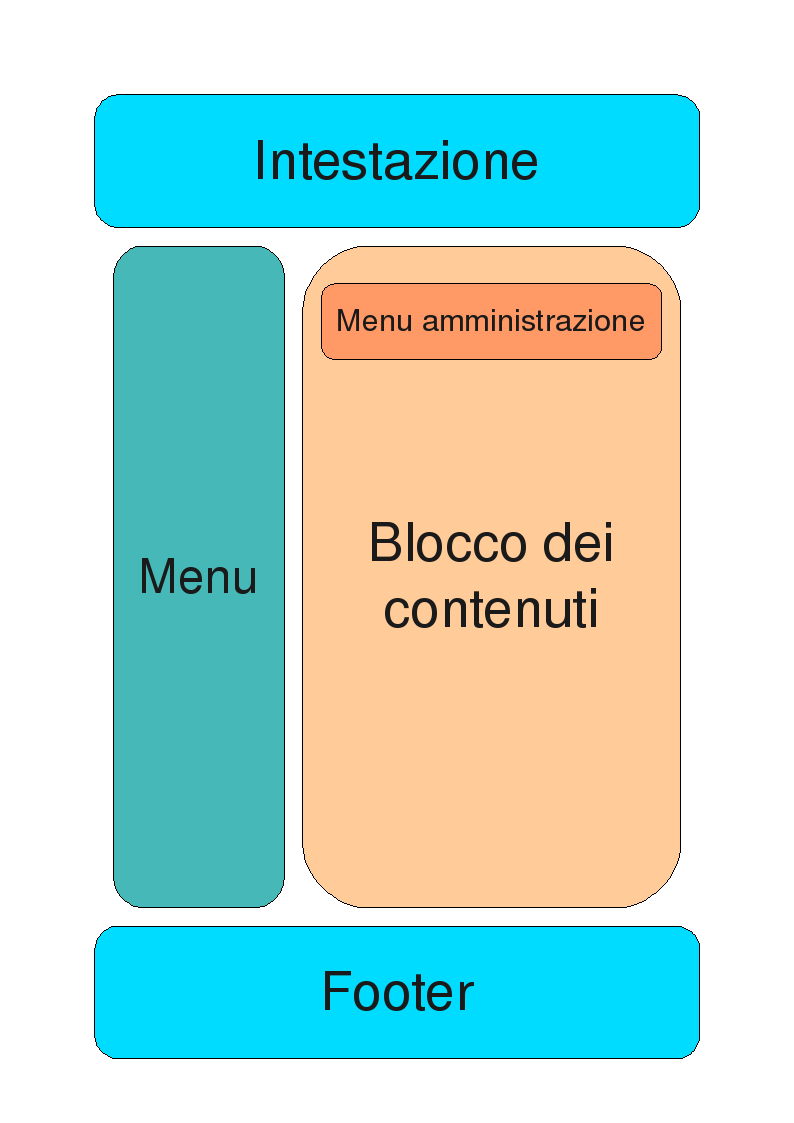
\includegraphics[scale=0.50]{images/layout.png}
\subsubsection{Templates}
Il sistema Sigeol prevede un diverso template per ogni azione raggiungibile attraverso una richiesta GET presente in ogni controller. Di seguito viene riportata una descrizione di ogni template:
\subsubsection*{Template comuni a più controller}
Per evitare fastidiose ripetizione di seguito sono riportate le descrizioni dei template per le azioni che figurano in più controller:
\begin{itemize}
 \item \verb|new.html.erb|: presenta un form per l'inserimento di una nuova istanza.
 \item \verb|edit.html.erb|: presenta un form per la modifica di un'istanza esistente.
 \item \verb|index.html.erb|: presenta un elenco ordinato di un insieme di istanze.
 \item \verb|show.html.erb|: presenta le informazioni relativa ad una determinata istanza.
 \item \verb|administration.html.erb|: presenta un elenco ordinato di un insieme di istanza e le relative funzioni
 per amministrarle.
 \item \verb|new_constraint.html.erb|: presenta un form per l'inserimento di un nuovo vincolo o preferenza
\end{itemize}
Inoltre per garantire l'interoperabilità dei dati sono presenti i template XML per tutte le azioni \verb|index| e \verb|show|, nonchè un template PDF per l'azione \verb|show| di \verb|TimetablesController|.
\subsubsection*{Template per TeachingsController}
Il template XHTML \verb|select_teacher.html.erb| è presente per il \\ \verb|TeachingsController| per l'azione \verb|select_teacher|.  Questo presenta un form per l'assegnamento di un docente ad un insegnamento utilizzando metodi per la presentazione automatica della lista dei docenti come i tag XHTML \verb|<select>| e \verb|<option>|.
\subsubsection*{Template per CurriculumsController}
Il template XHTML \verb|select_teaching.html.erb| è presente per il \\ \verb|CurriculumsController| per l'azione \verb|select_teaching|.  Questo presenta un form per l'assegnamento di un insegnamento ad un curriculum utilizzando metodi per la presentazione automatica della lista degli insegnamenti come i tag XHTML \verb|<select>| e \verb|<option>|.
\subsubsection*{Template per TeachersController}
Il \verb|TeachersController| prevede diverse azioni raggiungibili attraverso una richiesta GET ed i relativi template XHTML sono i seguenti:
\begin{itemize}
 \item \verb|pre_activate.html.erb|: presenta un form per l'attivazione dello \verb|user| del docente invitato
 \item \verb|edit_capabilities.html.erb|: presenta un form per l'assegnazione di nuovi privilegi allo \verb|user| detenuto dal docente utilizzando metodi per la presentazione automatica della lista dei privilegi come li tag XHTML \verb|<input type="checkbox">|
 \item \verb|edit_graduate_courses.html.erb|: presenta un form per l'assegnazione di nuovi corsi di laurea allo \verb|user| dtenuto dal docente utilizzando metodi per la presentazione automatica della lista dei corsi di laurea come i tag XHTML \verb|<select>| e \verb|<option>|
\end{itemize}
\subsubsection{Partials}
Il sistema Sigeol prevede l'uso di partials per la visualizzazione delle informazioni che sono riutilizzate in più view. Ognuno di essi è caratterizzato dalla presenza di un \_ (underscore) prima del nome del file che sono della forma \verb|_show_nomemodel.html.erb| e \verb|_show_nomemodel_admin.html.erb| e dovranno essere contenuti nella rispettiva directory che contiene i template del controller associato a \verb|nomemodel| (ad esempio \verb|_show_teaching.html.erb| è contenuto all'interno della directory \verb|app\view\teachings|. I partial del primo tipo visualizzano le informazioni dell'oggetto di tipo \verb|nomemodel| per le azioni di pubblico accesso, mentre i secondi per le azioni di amministrazione con le relative funzioni.

Per i controller che presentano l'azione \verb|administration| e necessitano di un menu di amministrazione è presente un partial \verb|_menu_admin.html.erb| per la visualizzazione del suddetto menu che risiederà nella stessa directory che contiene i template del controller in questione.

I partials, infine, che vengono utilizzati dal layout sono contenuti nella directory \verb|app\view\shared|, come ad esempio \verb|_user_sidebar.html.erb|.
\subsection{Componente Helper}\label{helper}
Il componente Helper si occupa di raccogliere le funzionalità di utilità necessarie ai componenti del pattern MVC. Ogni file che rappresenta un Helper non conterrà una classe, bensì un modulo, ovvero un insieme di metodi di pubblica utilità. Per ogni controller è previsto lo specifico Helper, anche se non è necessario che siano presenti dei metodi in quanto non tutti i controller (e le rispettive view) necessitano di funzioni ausiliarie.
\subsubsection{ApplicationHelper}
L' \verb|ApplicationHelper| contiene i metodi di utilità che non trovano una collocazione logica negli altri helper, nonchè tutte le funzionalità ausiliare richieste da più classi delle diverse componenti.
I metodi presenti all'interno dell' \verb|ApplicationHelper| sono i seguenti:
\begin{itemize}
 \item \verb|first_upper(name)|: metodo che restituisce la stringa \verb|name| a cui viene reso maiscolo il primo carattere e minuscoli i rimanenti.
 \item \verb|login_form|: metodo che \underline{renderizza} il partial per la form per il login.
 \item \verb|standard_sidebar|: metodo che renderizza il partial per il menu pubblico.
 \item \verb|user_sidebar|: metodo che renderizza il partial per il menu privato.
 \item \verb|link(user)|: metodo che restituisce l'insieme dei link disponibili per \verb|user|.
\end{itemize}
\subsubsection{BuildingsHelper}
I metodi presenti all'interno del \verb|BuildingsHelper| sono i seguenti:
\begin{itemize}
 \item \verb|menu_admin|: metodo che renderizza il partial per il menu di amministrazione per gli edifici.
 \item \verb|show_building_admin(building)|: metodo che renderizza il partial per l'amministrazione del \verb|building|.
 \item \verb|show_building(building)|: metodo che renderizza il partial per la visualizzazione del \verb|building|.
\end{itemize}
\subsubsection{ClassroomsHelper}
I metodi presenti all'interno del \verb|ClassroomsHelper| sono i seguenti:
\begin{itemize}
 \item \verb|menu_admin|: metodo che renderizza il partial per il menu di amministrazione per le aule.
 \item \verb|show_classroom_admin(classroom)|: metodo che renderizza il partial per l'amministrazione della \verb|classroom|.
\item \verb|show_classroom(classroom)|: metodo che renderizza il partial per la visualizzazione della \verb|classroom|.
\end{itemize}
\subsubsection{CurriculumsHelper}
I metodi presenti all'interno del \verb|CurriculumsHelper| sono i seguenti:
\begin{itemize}
\item \verb|show_curriculum_admin(curriculum)|: metodo che renderizza il partial per l'amministrazione del \verb|curriculum|.
\item \verb|show_curriculum(curriculum)|: metodo che renderizza il partial per la visualizzazione del \verb|curriculum|.
\end{itemize}
\subsubsection{SessionsHelper}
Non è presente nessun metodo all'interno di \verb|SessionsHelper|.
\subsubsection{GraduateCoursesHelper}
I metodi presenti all'interno del \verb|GraduateCoursesHelper| sono i seguenti:
\begin{itemize}
 \item \verb|menu_admin|: metodo che renderizza il partial per il menu di amministrazione per i corsi di laurea
 \item \verb|show_graduate_course_admin(graduate_course)|: metodo che renderizza il partial per l'amministrazione del  \verb|graduate_course|.
\item \verb|show_graduate_course(graduate_course)|: metodo che renderizza il partial per la visualizzazione del \verb|graduate_course|.
\end{itemize}
\subsubsection{TeachersHelper}
I metodi presenti all'interno del \verb|TeachersHelper| sono i seguenti:
\begin{itemize}
 \item \verb|menu_admin|: metodo che renderizza il partial per il menu di amministrazione per i docenti.
 \item \verb|show_teacher_admin(teacher)|: metodo che renderizza il partial per l'amministrazione del \verb|teacher|.
 \item \verb|show_teacher(teacher)|: metodo che renderizza il partial per la visualizzazione del \verb|teacher|.
\end{itemize}
\subsubsection{TeachingsHelper}
I metodi presenti all'interno del \verb|TeachingsHelper| sono i seguenti:
\begin{itemize}
 \item \verb|menu_admin|: metodo che renderizza il partial per il menu di amministrazione per gli insegnamenti.
 \item \verb|show_teaching_admin(teaching)|: metodo che renderizza il partial per l'amministrazione del \verb|teaching|.
 \item \verb|show_teaching(teaching)|: metodo che renderizza il partial per la visualizzazione del \verb|teaching|.
\end{itemize}
\subsubsection{TimetablesHelper}
I metodi presenti all'interno del \verb|TimetablesHelper| sono i seguenti:
\begin{itemize}
 \item \verb|menu_admin|: metodo che renderizza il partial per il menu di amministrazione per gli orari.
 \item \verb|show_timetable_admin(timetable)|: metodo che renderizza il partial per l'amministrazione del \verb|timetable|.
 \item \verb|show_timetable(timetable)|: metodo che renderizza il partial per la visualizzazione del \verb|timetable|.
\end{itemize}
\subsubsection{UsersHelper}
I metodi presenti all'interno del \verb|UsersHelper| sono i seguenti:
\begin{itemize}
 \item \verb|show_not_active_users(user)|: metodo che renderizza il partial per la visualizzazione dello \verb|user| non ancora attivo.
\end{itemize}
\modifiche
\end{document}
